\chapter{DevOps}\label{ch-10}

\lecturemeta{Capitolo originale: 10 --- DevOps \quad\textbullet\quad Antonio Brogi}{Appunti di Emiliano Sescu (github.com/Faxatos), cap. 10}

Nell'ingegneria del software project-based c'erano due team separati:

\begin{itemize}
\tightlist
\item
  un \textbf{team di sviluppo}, che si occupava di tutto lo sviluppo
  (design, requisiti, specifiche, prototipi, test, integrazione) fino a
  consegnare un software testato e pronto al rilascio;
\item
  un \textbf{team operativo} (\emph{operations}), che installava e
  manteneva il sistema (supporto agli utenti ed eventuali modifiche al
  software).
\end{itemize}

I problemi di questo modello erano i ritardi di comunicazione tra i
team, strumenti diversi, competenze diverse e spesso la difficoltà a
capire i problemi dell'altro team. In più, per correggere bug urgenti o
vulnerabilità di sicurezza servivano giorni, perché il team operativo
non aveva sviluppato il software.

Tre fattori hanno permesso il cambiamento:

\begin{itemize}
\tightlist
\item
  l'\textbf{ingegneria del software Agile} ha ridotto i tempi di
  sviluppo, e il processo di rilascio tradizionale è diventato un collo
  di bottiglia;
\item
  \textbf{Amazon} ha riprogettato il suo software a (micro)servizi,
  affidando sviluppo e supporto di ogni servizio \textbf{allo stesso
  team};
\item
  è diventato possibile rilasciare software come \textbf{SaaS} su cloud
  pubblici o privati.
\end{itemize}

\begin{boxdefinition}{DevOps}

Il \textbf{DevOps} (\emph{Development} + \emph{Operations}) unisce
sviluppo, deploy e supporto in \textbf{un unico team}.

\end{boxdefinition}

I principi del DevOps sono:

\begin{itemize}
\tightlist
\item
  \textbf{Tutti sono responsabili di tutto}: tutti i membri del team
  condividono la responsabilità di sviluppare, rilasciare e supportare
  il software.
\item
  \textbf{Tutto ciò che si può automatizzare va automatizzato}: tutte (o
  quasi) le attività di test, deploy e supporto devono essere
  automatiche.
\item
  \textbf{Prima misura, poi cambia}: il DevOps deve essere guidato dai
  dati raccolti sul sistema e sul suo funzionamento.
\end{itemize}

Vantaggi del DevOps:

\begin{itemize}
\tightlist
\item
  \textbf{Deploy più veloce} (il vantaggio principale): i ritardi di
  comunicazione tra persone si riducono drasticamente, e si passa in
  produzione in ore invece che in giorni o settimane.
\item
  \textbf{Meno rischi}: ogni release aggiunge piccoli incrementi di
  funzionalità, quindi ci sono meno probabilità di interazioni
  impreviste tra feature e di guasti.
\item
  \textbf{Riparazioni più rapide}: non bisogna scoprire quale team deve
  risolvere il problema e aspettare che lo faccia.
\item
  \textbf{Team più produttivi}: i team DevOps sono più produttivi di
  team che si occupano di attività separate.
\end{itemize}

Un team DevOps mette insieme competenze diverse: ingegneria del
software, UX design, sicurezza, infrastruttura, rapporto con i clienti e
altro. Il suo successo si basa su:

\begin{itemize}
\tightlist
\item
  una \textbf{cultura di rispetto reciproco e condivisione}: tutti
  partecipano agli scrum e alle altre riunioni, e ognuno è incoraggiato
  a condividere le proprie competenze e a impararne di nuove;
\item
  il \textbf{supporto degli sviluppatori al software che hanno scritto}:
  se un servizio si guasta nel weekend, è lo sviluppatore che deve
  rimetterlo in funzione; se non è disponibile, lo fa un altro membro
  del team. I team DevOps puntano a riparare i guasti il più in fretta
  possibile, \textbf{non a cercare un colpevole}.
\end{itemize}

\section{Gestione del codice}\label{gestione-del-codice}

Durante lo sviluppo di un prodotto si scrivono decine di migliaia di
righe di codice e di test automatici, organizzate in centinaia di file.
Si usano decine di librerie e servono vari programmi per creare ed
eseguire il codice: senza un supporto automatico è impossibile tenere
traccia delle modifiche.

\begin{boxdefinition}{Sistema di gestione del codice}

Un \textbf{code management system} è un software che supporta le
pratiche per gestire un codice che evolve nel tempo. Deve garantire che
le modifiche di sviluppatori diversi \textbf{non interferiscano} tra
loro e aiutare a creare \textbf{versioni diverse} del prodotto. Deve
anche semplificare la creazione del prodotto eseguibile dai sorgenti e
l'esecuzione dei test automatici.

\end{boxdefinition}

La Fig. 10.1 mostra i componenti: in alto la pipeline \textbf{CI/CD}
(\emph{Continuous Integration / Continuous Delivery-Deployment}), in
basso le \textbf{misurazioni DevOps}, al centro il sistema di gestione
del codice con le sue funzionalità principali.

\begin{figure}[H]
\centering
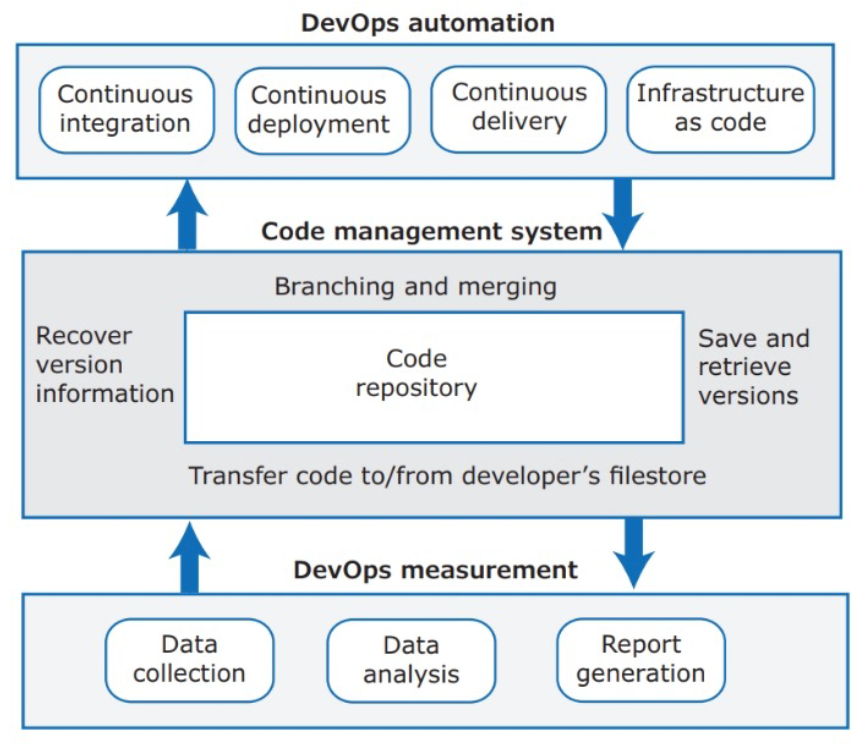
\includegraphics[width=0.75\linewidth,height=0.45\textheight,keepaspectratio]{images/10-devops_fig10-1_struttura-devops.png}
\caption{La struttura di un sistema DevOps.}
\end{figure}

Funzionalità di un sistema di gestione del codice:

\begin{itemize}
\tightlist
\item
  \textbf{Identificazione di versioni e release}: ogni versione di un
  file inviata al sistema riceve un identificatore unico (i file gestiti
  non vengono mai sovrascritti) e si può recuperare con l'identificatore
  o con altri attributi del file.
\item
  \textbf{Registrazione della storia delle modifiche}: chi invia una
  modifica deve aggiungere una nota che ne spiega il motivo, così gli
  altri capiscono perché è nata una nuova versione.
\item
  \textbf{Sviluppo indipendente}: più sviluppatori possono lavorare
  sullo stesso file contemporaneamente. Ogni invio crea una nuova
  versione, quindi i file non vengono mai sovrascritti da modifiche
  successive.
\item
  \textbf{Supporto ai progetti}: gli sviluppatori scaricano il codice
  nel loro spazio personale, ci lavorano e lo rimandano al sistema
  condiviso. Si possono creare \textbf{branch} paralleli per lavorare in
  contemporanea, e le modifiche fatte in branch diversi si possono unire
  (\textbf{merge}). Tutti i file di un progetto si possono scaricare
  insieme.
\item
  \textbf{Gestione dello spazio}: meccanismi efficienti evitano di
  tenere più copie di file che differiscono di poco (oggi meno
  importante, perché lo spazio costa poco).
\end{itemize}

\subsection{Sistemi centralizzati e
distribuiti}\label{sistemi-centralizzati-e-distribuiti}

All'inizio si usavano sistemi \textbf{centralizzati}, ma i vantaggi dei
sistemi \textbf{distribuiti} (es. \textbf{Git}, creato per il kernel
Linux) li hanno resi la soluzione migliore:

\begin{itemize}
\tightlist
\item
  \textbf{Resilienza}: ognuno ha la propria copia del repository (e può
  lavorare anche offline). Se il repository condiviso si danneggia o
  viene attaccato, si continua a lavorare e lo si ripristina dalle
  copie.
\item
  \textbf{Velocità}: fare commit è veloce, perché si può fare in locale
  (senza trasferire dati in rete) oltre che sul branch comune.
\item
  \textbf{Flessibilità}: avendo ognuno la propria copia, sperimentare in
  locale è molto più semplice e sicuro.
\end{itemize}

In Git ogni sviluppatore ha sul proprio computer un \textbf{clone
privato} del repository condiviso, e c'è un \textbf{repository di
progetto condiviso} (sul server dell'azienda o nel cloud, su servizi
come GitHub o GitLab). La Fig. 10.2 mostra alcuni comandi Git e
l'aspetto dei branch.

\begin{figure}[H]
\centering
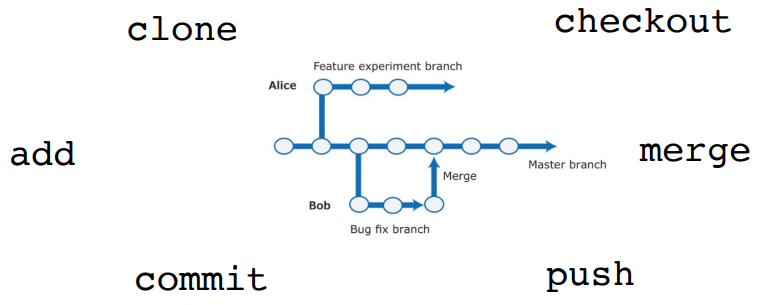
\includegraphics[width=1.00\linewidth,height=0.45\textheight,keepaspectratio]{images/10-devops_fig10-2_branch-git.png}
\caption{Esempio di branch Git.}
\end{figure}

\begin{boxtip}{I comandi Git della figura}

\begin{itemize}
\tightlist
\item
  \texttt{clone}: copia in locale un repository remoto.
\item
  \texttt{add}: prepara le modifiche da salvare (le mette nella
  \emph{staging area}).
\item
  \texttt{commit}: salva le modifiche preparate come nuova versione nel
  repository locale.
\item
  \texttt{push}: invia i commit locali al repository condiviso.
\item
  \texttt{checkout}: passa a un altro branch o a un'altra versione.
\item
  \texttt{merge}: unisce le modifiche di un branch in un altro.
\end{itemize}

\end{boxtip}

Nello sviluppo open source con Git di solito c'è un gruppo di persone
che decide quali modifiche accettare. GitHub usa un meccanismo chiamato
\textbf{Webhooks} per avviare gli strumenti di automazione DevOps quando
il repository del progetto viene aggiornato.

\section{Automazione DevOps}\label{automazione-devops}

``\textbf{Tutto ciò che si può automatizzare va automatizzato}'':
vediamo nel dettaglio questo principio del DevOps. Le forme di
automazione sono:

\begin{itemize}
\tightlist
\item
  \textbf{Continuous integration}: ogni volta che uno sviluppatore fa
  commit di una modifica sul branch principale (\emph{master}), si
  costruisce e si testa una versione eseguibile del sistema.
\item
  \textbf{Continuous delivery}: costruita la nuova versione, il software
  eseguibile viene testato in un ambiente che simula quello operativo
  del prodotto.
\item
  \textbf{Continuous deployment}: una nuova release del sistema viene
  resa disponibile agli utenti ogni volta che si fa una modifica al
  branch principale.
\item
  \textbf{Infrastructure as code}: modelli leggibili dalle macchine
  dell'infrastruttura su cui gira il prodotto (rete, server, router,
  \ldots) vengono usati da strumenti di gestione della configurazione
  per costruire la piattaforma di esecuzione. Il modello include anche
  il software da installare (compilatori, librerie, DBMS, \ldots).
\end{itemize}

\subsection{Continuous integration}\label{continuous-integration}

Serve la continuous integration perché, se il sistema si integra
raramente, i problemi sono \textbf{difficili da isolare} e correggerli
rallenta lo sviluppo. Integrare il sistema (\emph{system building}) non
vuol dire solo compilare, ma anche:

\begin{enumerate}
\def\labelenumi{\arabic{enumi}.}
\tightlist
\item
  installare il software del database e creare il database con lo schema
  giusto;
\item
  caricare nel database i dati di test;
\item
  collegare il codice compilato con le librerie e gli altri componenti
  usati;
\item
  controllare che i servizi esterni usati siano attivi;
\item
  spostare i file di configurazione nelle posizioni giuste (e cancellare
  quelli vecchi);
\item
  eseguire i test di sistema per controllare che l'integrazione sia
  riuscita.
\end{enumerate}

Come mostra la Fig. 10.3, ogni volta che si fa push di una modifica sul
repository condiviso si crea e si testa una versione integrata del
sistema. Finito il push, il repository manda un messaggio al
\textbf{server di integrazione}, che costruisce una nuova versione del
prodotto.

\begin{figure}[H]
\centering
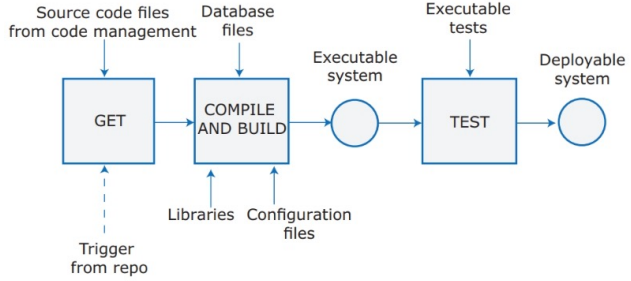
\includegraphics[width=0.80\linewidth,height=0.45\textheight,keepaspectratio]{images/10-devops_fig10-3_pipeline-ci.png}
\caption{La pipeline di continuous integration.}
\end{figure}

\begin{boxtip}{Integrate twice}

È buona pratica \textbf{integrare due volte}: prima sulla macchina
locale dello sviluppatore, poi facendo push sul repository del progetto,
che avvia il server di integrazione (Fig. 10.4). Si fa così perché
mettere una \textbf{build rotta} nel repository di progetto è una cosa
molto grave.

\end{boxtip}

\begin{figure}[H]
\centering
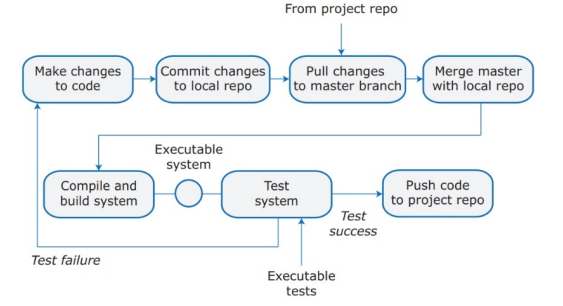
\includegraphics[width=0.80\linewidth,height=0.45\textheight,keepaspectratio]{images/10-devops_fig10-4_integrate-twice.png}
\caption{La pipeline ``integrate twice''.}
\end{figure}

Vantaggi della continuous integration:

\begin{itemize}
\tightlist
\item
  \textbf{Trovare e correggere i bug è più veloce}: se si fa una piccola
  modifica e un test di sistema fallisce, il problema è quasi certamente
  nel nuovo codice.
\item
  \textbf{C'è sempre un sistema funzionante} a disposizione del team,
  per provare idee e fare demo al management e ai clienti.
\item
  \textbf{Cultura della qualità} nel team: nessuno vuole essere quello
  che ha ``rotto la build'', quindi tutti controllano bene il proprio
  lavoro prima del push.
\end{itemize}

Analizzare tutto il codice a ogni commit è molto pesante: per questo gli
strumenti di integrazione \textbf{ripetono le operazioni solo se i file
da cui dipendono sono cambiati} (es. ricompilano solo i file sorgente
modificati). Per capire se una dipendenza è cambiata si possono usare le
\textbf{date di modifica} dei file.

\subsection{Continuous delivery e
deployment}\label{continuous-delivery-e-deployment}

Con la continuous integration e la gestione del codice si può creare una
versione eseguibile del sistema, costruendolo e testandolo prima sul
computer dello sviluppatore e poi sul server di integrazione.

Quando però lo si installa nell'\textbf{ambiente di produzione reale},
qualcosa può andare storto, perché la produzione è \textbf{diversa
dall'ambiente di sviluppo} (il server può avere un'organizzazione del
file system diversa, permessi diversi, applicazioni installate diverse,
\ldots).

La \textbf{continuous delivery} garantisce che il sistema modificato sia
pronto per i clienti eseguendo test delle feature nell'ambiente di
produzione (per controllare che l'ambiente non causi guasti), test di
sistema e \textbf{test di carico} (per vedere come si comporta il
software quando aumentano gli utenti). Il modo più semplice per creare
una replica dell'ambiente di produzione sono i \textbf{container}.

Come mostra la Fig. 10.5:

\begin{itemize}
\tightlist
\item
  per la \textbf{delivery}, dopo i primi test di integrazione si
  configura un ambiente di test ``a fasi'' (\emph{staged}) e si lanciano
  i test di accettazione del sistema (funzionalità, carico,
  prestazioni);
\item
  per il \textbf{deployment}, software e dati vengono trasferiti sui
  server di produzione, si passa alla nuova versione del sistema e si
  riavvia il processo. È fondamentale gestire anche i client ancora
  collegati alla vecchia versione.
\end{itemize}

\begin{figure}[H]
\centering
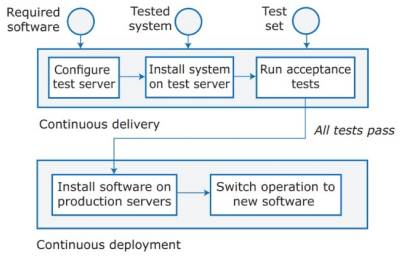
\includegraphics[width=0.60\linewidth,height=0.45\textheight,keepaspectratio]{images/10-devops_fig10-5_delivery-deployment.png}
\caption{Schema di continuous delivery e continuous deployment.}
\end{figure}

\begin{boxtip}{Delivery vs deployment}

Con la \textbf{continuous delivery} il software è sempre \textbf{pronto}
per essere rilasciato (ma la decisione di rilasciarlo può restare
manuale). Con il \textbf{continuous deployment} ogni modifica che passa
i test viene \textbf{rilasciata automaticamente} agli utenti.

\end{boxtip}

Vantaggi del continuous deployment:

\begin{itemize}
\tightlist
\item
  \textbf{Costi ridotti}: la pipeline di deploy è completamente
  automatica.
\item
  \textbf{Problemi risolti più in fretta}: un problema probabilmente
  riguarda una piccola parte del sistema, e la sua causa è evidente.
\item
  \textbf{Feedback dei clienti più rapido}: si rilasciano le nuove
  feature appena sono pronte e si usa il feedback degli utenti per
  migliorarle.
\item
  \textbf{A/B testing}: con molti clienti e più server, si può
  installare la nuova versione solo su alcuni server e usare un load
  balancer per mandarci una parte dei clienti, così si misura come
  vengono usate le nuove feature.
\end{itemize}

\begin{boxwarning}{Non rilasciare proprio tutto}

Probabilmente conviene non rilasciare ogni singola modifica:

\begin{itemize}
\tightlist
\item
  piccole modifiche possono contenere feature incomplete, che è meglio
  non mostrare ai concorrenti prima di averle finite;
\item
  i clienti possono irritarsi se il software cambia di continuo,
  soprattutto l'interfaccia;
\item
  si possono voler sincronizzare i rilasci con i cicli di business noti
  (es. l'inizio dell'anno scolastico per il mercato dell'istruzione).
\end{itemize}

\end{boxwarning}

Molti strumenti di continuous integration (come \textbf{Jenkins} e
\textbf{Travis}) si possono usare anche per la continuous delivery e il
deployment. Si possono integrare con strumenti di gestione della
configurazione dell'infrastruttura, anche se per il software nel cloud
spesso è più semplice usare i \textbf{container} insieme agli strumenti
di CI.

\subsection{Infrastructure as code}\label{infrastructure-as-code}

Gestire a mano un'infrastruttura con decine o centinaia di server è
\textbf{costoso e soggetto a errori}. I server (fisici o virtuali) hanno
configurazioni diverse e software diversi: quando esce una nuova
versione di un software, alcuni server vanno aggiornati e altri no, per
via di dipendenze da versioni vecchie. Tenere traccia a mano del
software installato su ogni server è difficilissimo e spesso non si fa
(es. le modifiche d'emergenza non sempre vengono documentate).

L'idea è automatizzare l'aggiornamento dei server usando un
\textbf{modello dell'infrastruttura leggibile dalle macchine}. Gli
strumenti di \textbf{Configuration Management} (CM, come
\textbf{Puppet}, \textbf{Chef} e \textbf{Ansible}) installano
automaticamente software e servizi sui server secondo la definizione
dell'infrastruttura. L'infrastruttura è rappresentata come dati, per
questo si parla di \textbf{Infrastructure as Code} (IaC, Fig. 10.6).
Quando serve un cambiamento si aggiorna il modello, e lo strumento CM
applica le modifiche a tutti i server.

\begin{figure}[H]
\centering
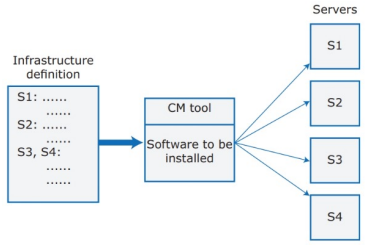
\includegraphics[width=0.60\linewidth,height=0.45\textheight,keepaspectratio]{images/10-devops_fig10-6_infrastructure-as-code.png}
\caption{Schema dell'infrastructure as code.}
\end{figure}

Vantaggi dell'infrastructure as code:

\begin{itemize}
\tightlist
\item
  \textbf{Visibilità}: l'infrastruttura è definita in un modello a sé
  che tutto il team DevOps può leggere, capire e revisionare.
\item
  \textbf{Riproducibilità}: le installazioni avvengono sempre nella
  stessa sequenza e producono sempre lo stesso ambiente. Non serve che
  qualcuno si ricordi l'ordine delle operazioni (i computer sono più
  affidabili delle persone in questo).
\item
  \textbf{Affidabilità}: l'automazione evita i piccoli errori che gli
  amministratori fanno quando ripetono le stesse modifiche su più
  server.
\item
  \textbf{Ripristino}: il modello dell'infrastruttura si può versionare
  e salvare nel sistema di gestione del codice. Se una modifica crea
  problemi, si torna facilmente a una versione precedente e si
  reinstalla l'ambiente che si sa funzionare.
\end{itemize}

I \textbf{container} sono un modo molto efficace per rilasciare prodotti
nel cloud, perché rendono semplice avere \textbf{ambienti di esecuzione
identici}: per ogni tipo di server si definisce l'ambiente necessario e
si costruisce un'immagine; quando si aggiorna il software si crea una
nuova immagine. Per scalabilità, resilienza e orchestrazione si può
usare un sistema di gestione dei container come \textbf{Kubernetes}
(vedi \href{05\%20-\%20Software\%20cloud-based}{05 - Software
cloud-based}).

\section{Misurazioni DevOps}\label{misurazioni-devops}

Per migliorare continuamente il processo DevOps, cioè rilasciare più in
fretta software di qualità migliore, bisogna \textbf{misurare e
analizzare} dati sul prodotto e sul processo. Ci sono vari tipi di
misurazioni:

\begin{itemize}
\tightlist
\item
  \textbf{Misure di processo}: dati sui processi di sviluppo, test e
  deploy.
\item
  \textbf{Misure di servizio}: dati su prestazioni, affidabilità e
  gradimento del software da parte dei clienti.
\item
  \textbf{Misure d'uso}: dati su \textbf{come i clienti usano} il
  prodotto (invece di mostrare pop-up che chiedono se il prodotto è
  piaciuto); aiutano a trovare problemi nel software stesso.
\item
  \textbf{Misure di successo del business}: dati su quanto il prodotto
  contribuisce al successo complessivo dell'azienda. È difficile isolare
  il contributo del DevOps, perché il successo potrebbe dipendere dal
  DevOps oppure da una gestione migliore.
\end{itemize}

\begin{boxexample}{Metriche tipiche}

\begin{itemize}
\tightlist
\item
  \textbf{Processo}: frequenza dei deploy, percentuale di deploy
  falliti, tempo medio di ripristino dopo un guasto.
\item
  \textbf{Servizio}: disponibilità, tempi di risposta, numero di
  segnalazioni dei clienti.
\item
  \textbf{Uso}: numero di utenti attivi, feature più e meno usate,
  durata delle sessioni.
\end{itemize}

\end{boxexample}

Misurare il software e il suo sviluppo è complesso: bisogna scegliere
metriche che diano informazioni utili e trovare modi affidabili per
raccoglierle e analizzarle. Alcune misure (es. la \textbf{soddisfazione
dei clienti}) vanno ricavate da altre metriche (es. il \textbf{numero di
clienti che tornano}).

La misurazione va automatizzata il più possibile: gli sviluppatori
devono \textbf{strumentare} il software perché raccolga dati su se
stesso e usare un sistema di monitoraggio per le prestazioni e la
disponibilità. Per raccogliere dati in automatico si può:

\begin{itemize}
\tightlist
\item
  usare strumenti di continuous integration come \textbf{Jenkins} per i
  dati su deploy, test superati, ecc.;
\item
  usare i servizi di monitoraggio dei provider cloud, come
  \textbf{Amazon CloudWatch}, per disponibilità e prestazioni;
\item
  raccogliere i dati forniti dai clienti tramite i sistemi di gestione
  delle segnalazioni (\emph{issue management});
\item
  aggiungere al prodotto della \textbf{strumentazione} per raccogliere
  dati sulle prestazioni e su come lo usano i clienti. Di solito i
  \textbf{file di log} sono la scelta migliore: si registrano più eventi
  possibile e si usano strumenti di analisi dei log per capire come
  viene usato il software.
\end{itemize}
